\documentclass{article}
\usepackage{graphicx} % Required for inserting images
\usepackage{geometry} % Required for adjusting margins

% Adjust margins to be as small as possible
\geometry{
    a4paper,          % Use A4 paper size
    left=10mm,        % Left margin
    right=10mm,       % Right margin
    top=10mm,         % Top margin
    bottom=10mm       % Bottom margin
}

\begin{document}

% Title Section
\title{UML Diagram for CC3K+}
\author{Jian Feng}
\date{\today}
\maketitle

% Main Content
\section{UML Diagram}
From the initial design to the final implementation, my design maintained the original core structure and concept, without refactoring or significantly modifying the original class model. All new functions and features were implemented by adding new methods and fields to ensure compatibility and consistency with the existing design.
% Figure Section
\begin{figure}[htbp]
    \centering
    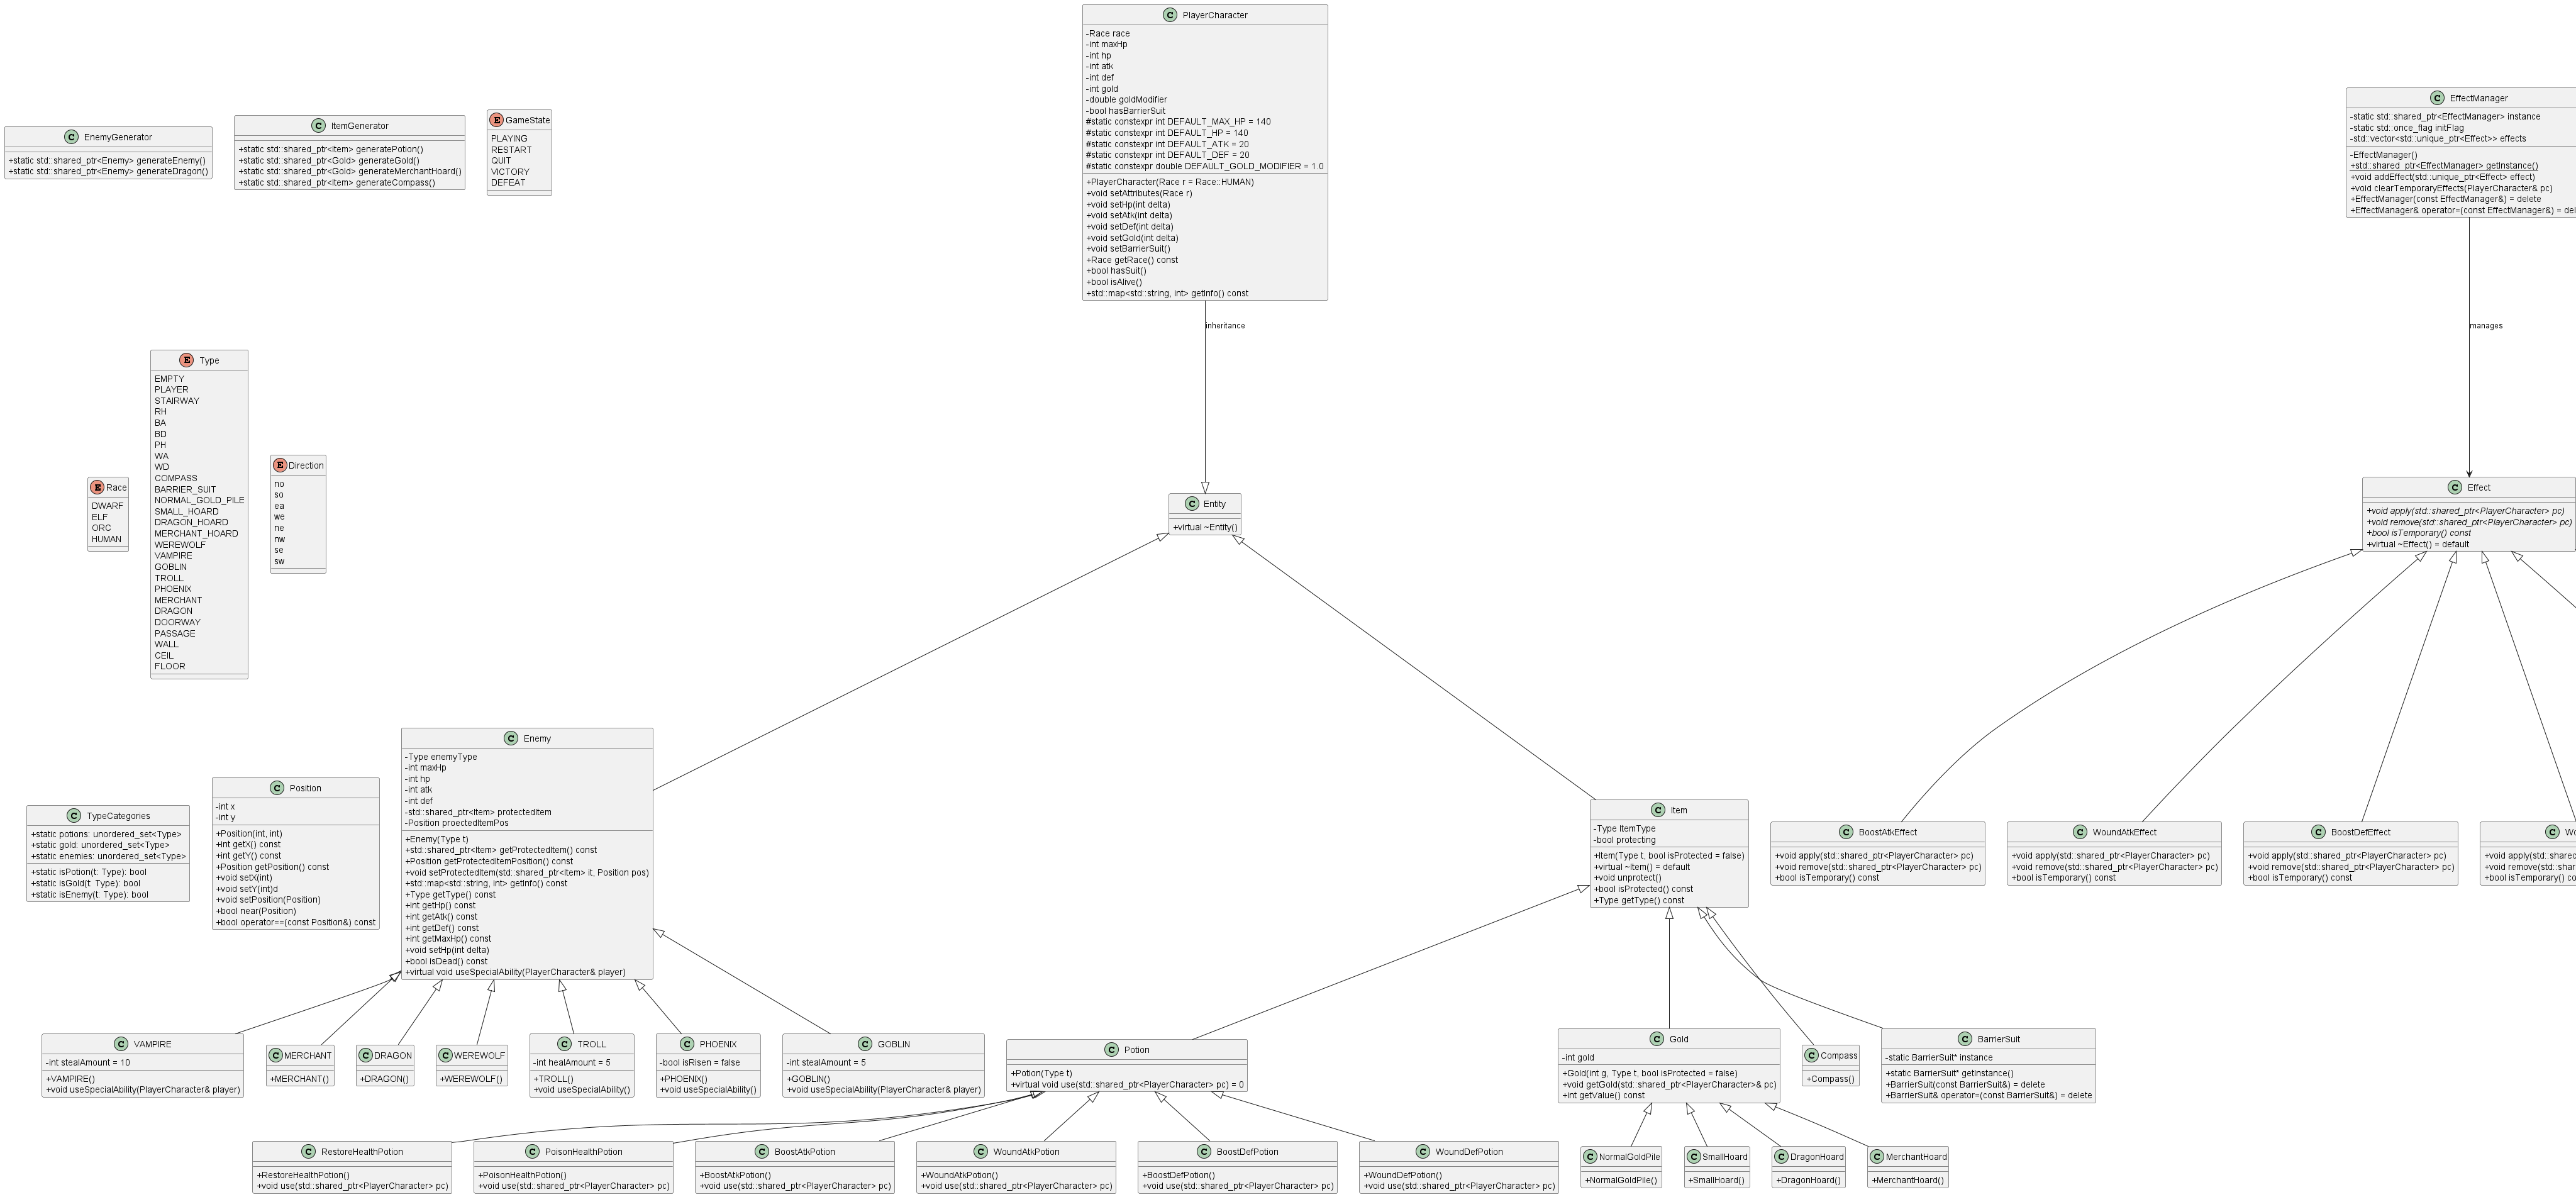
\includegraphics[width=\linewidth]{./out/uml_v0/uml_v0.png} % Use full line width
    \caption{UML Diagram v0}
    \label{fig:uml-diagram-0}
\end{figure}

\begin{figure}[htbp]
    \centering
    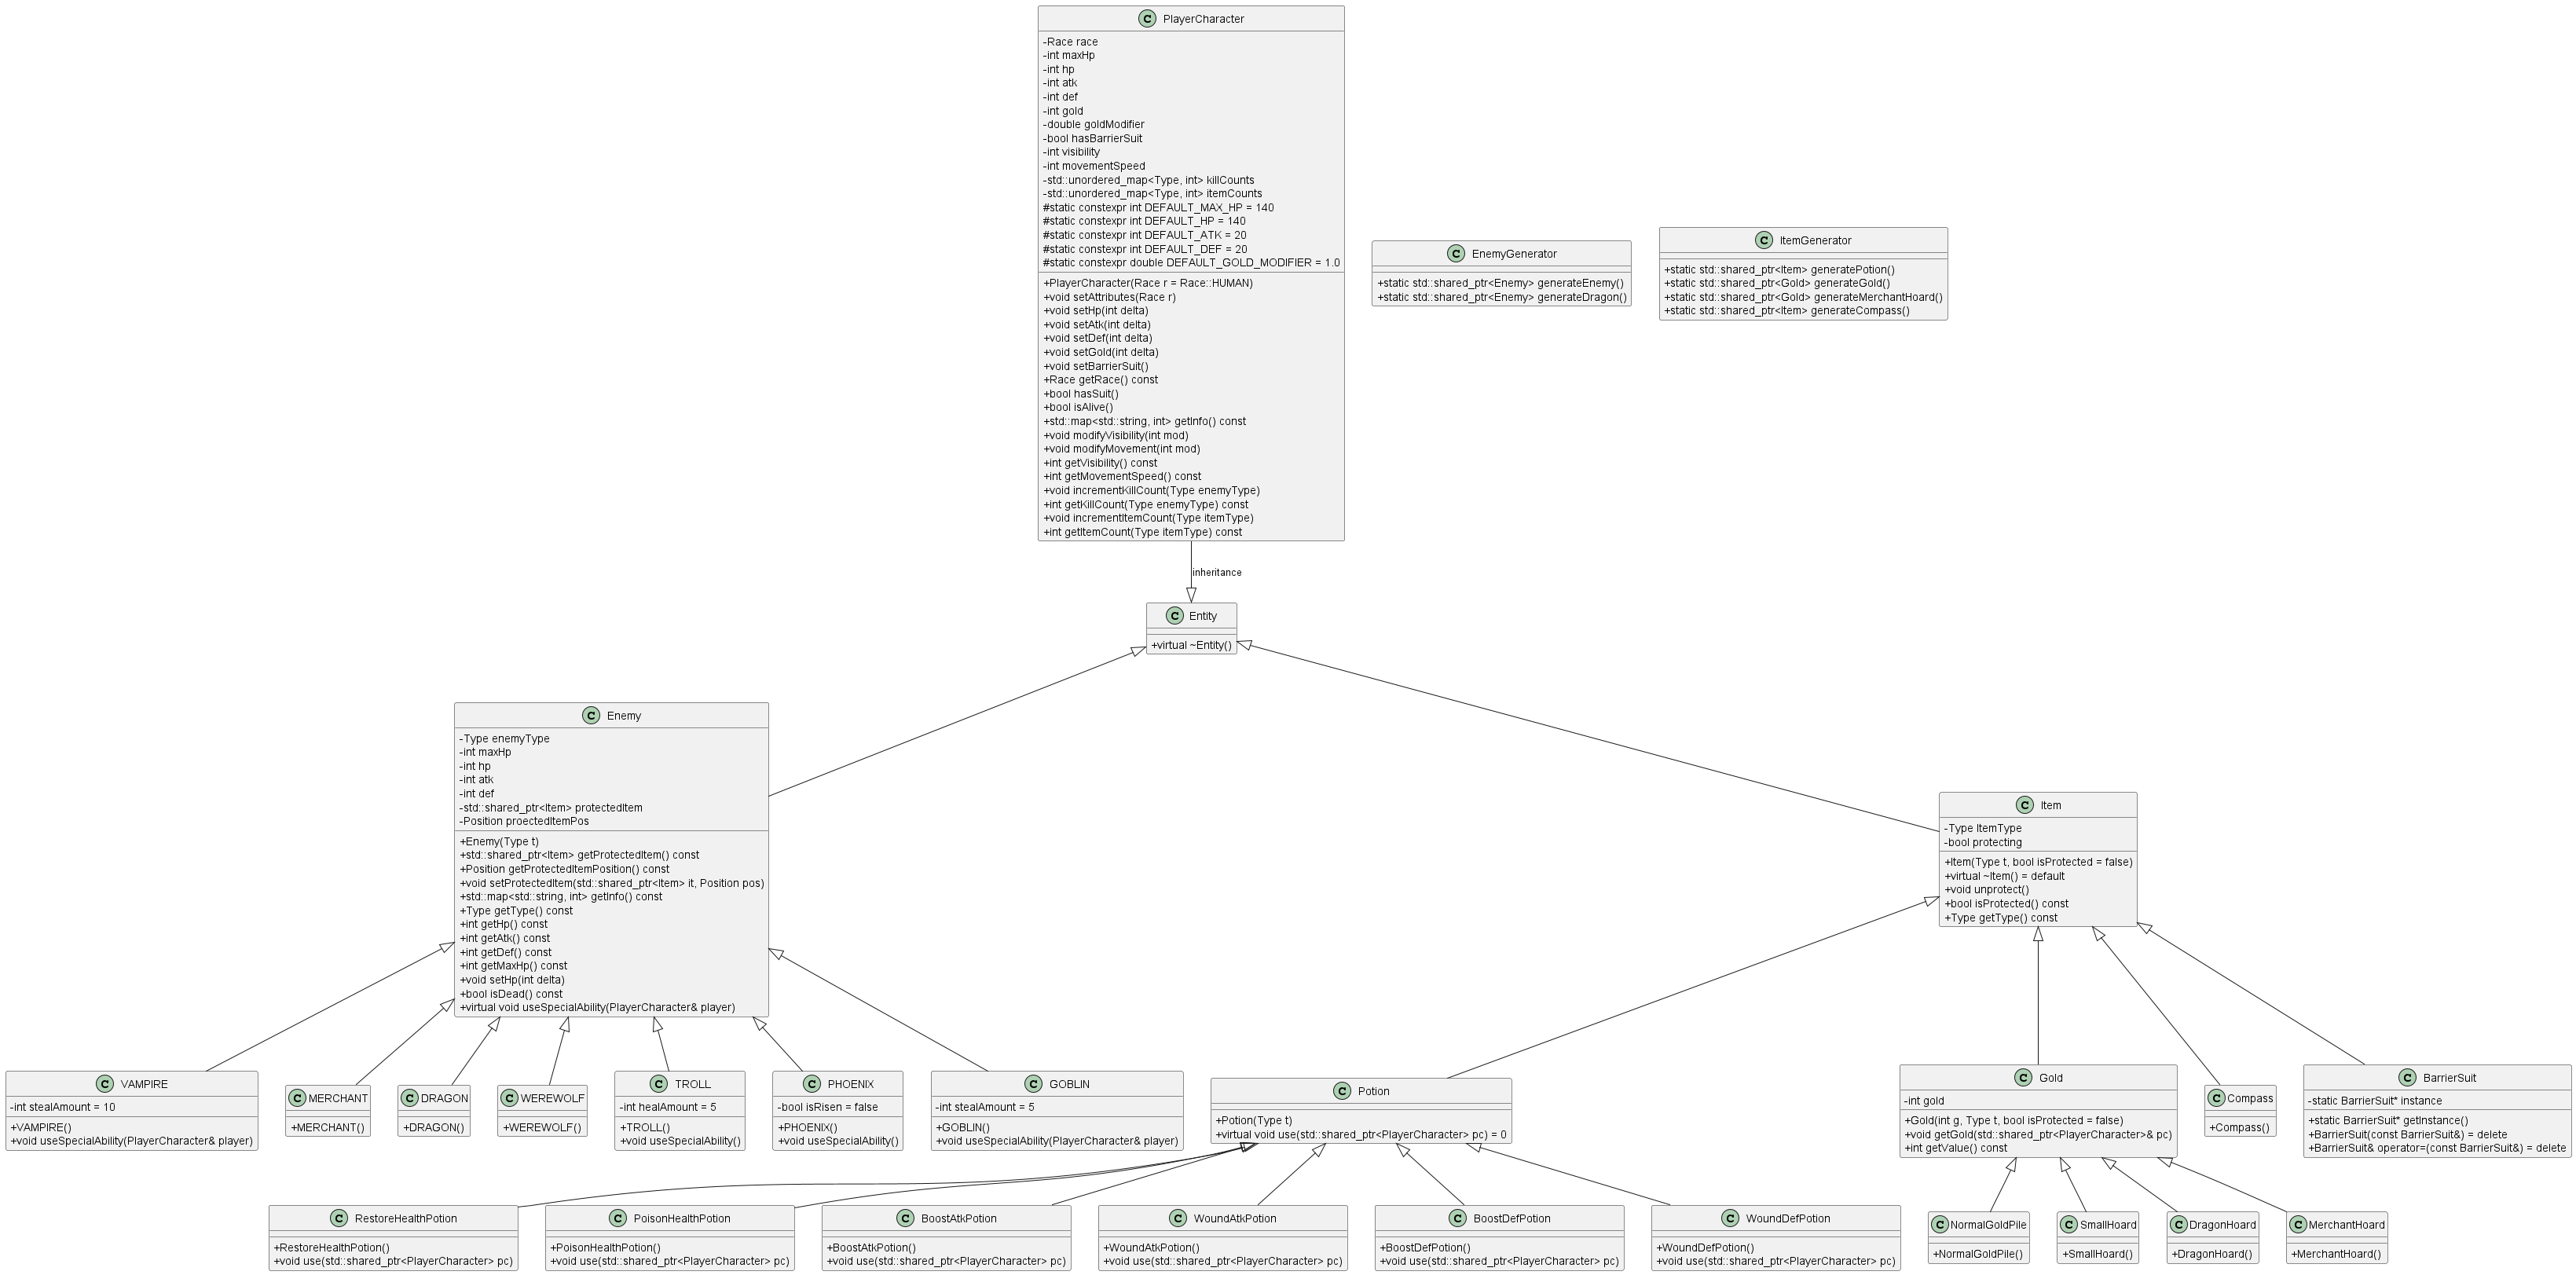
\includegraphics[width=\linewidth]{./out/uml_v1/uml1.png} % Use full line width
    \caption{UML Diagram-1 v1}
    \label{fig:uml-diagram-1}
\end{figure}
\begin{figure}[htbp]
    \centering
    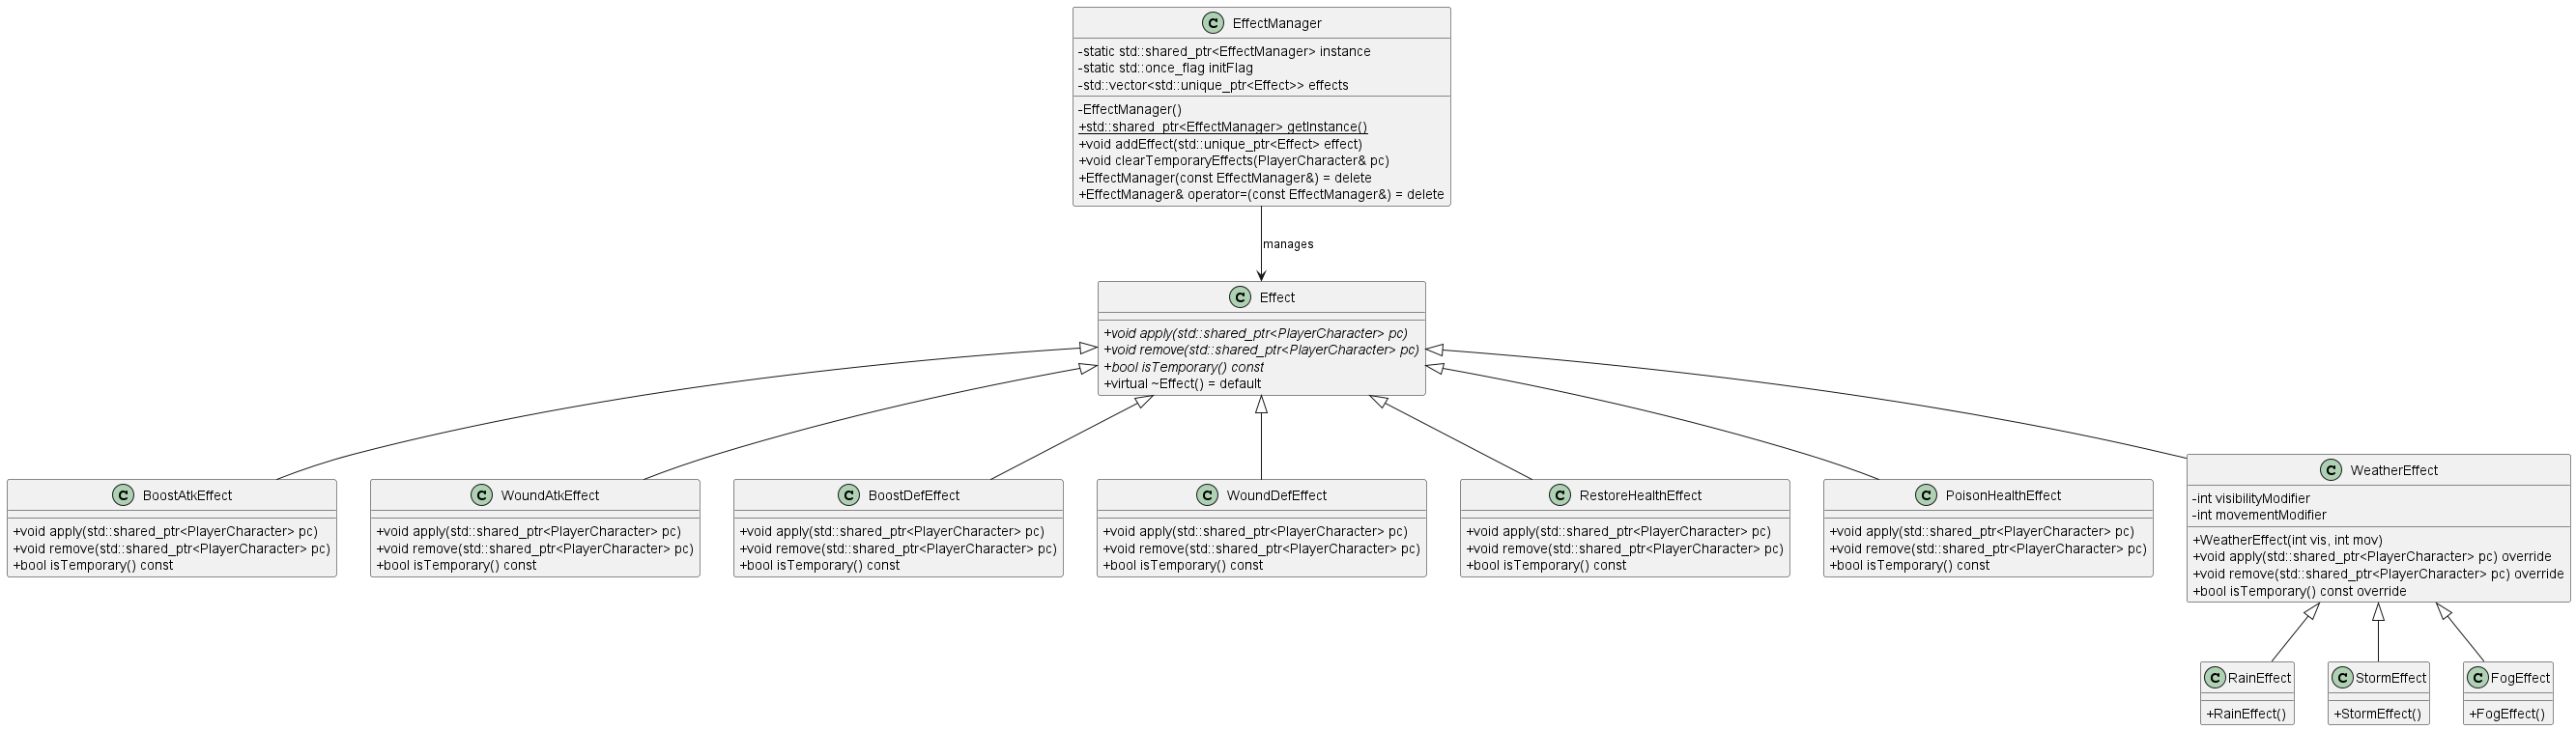
\includegraphics[width=\linewidth]{./out/uml_v1/uml2.png} % Use full line width
    \caption{UML Diagram-2 v1}
    \label{fig:uml-diagram-2}
\end{figure}
\begin{figure}[htbp]
    \centering
    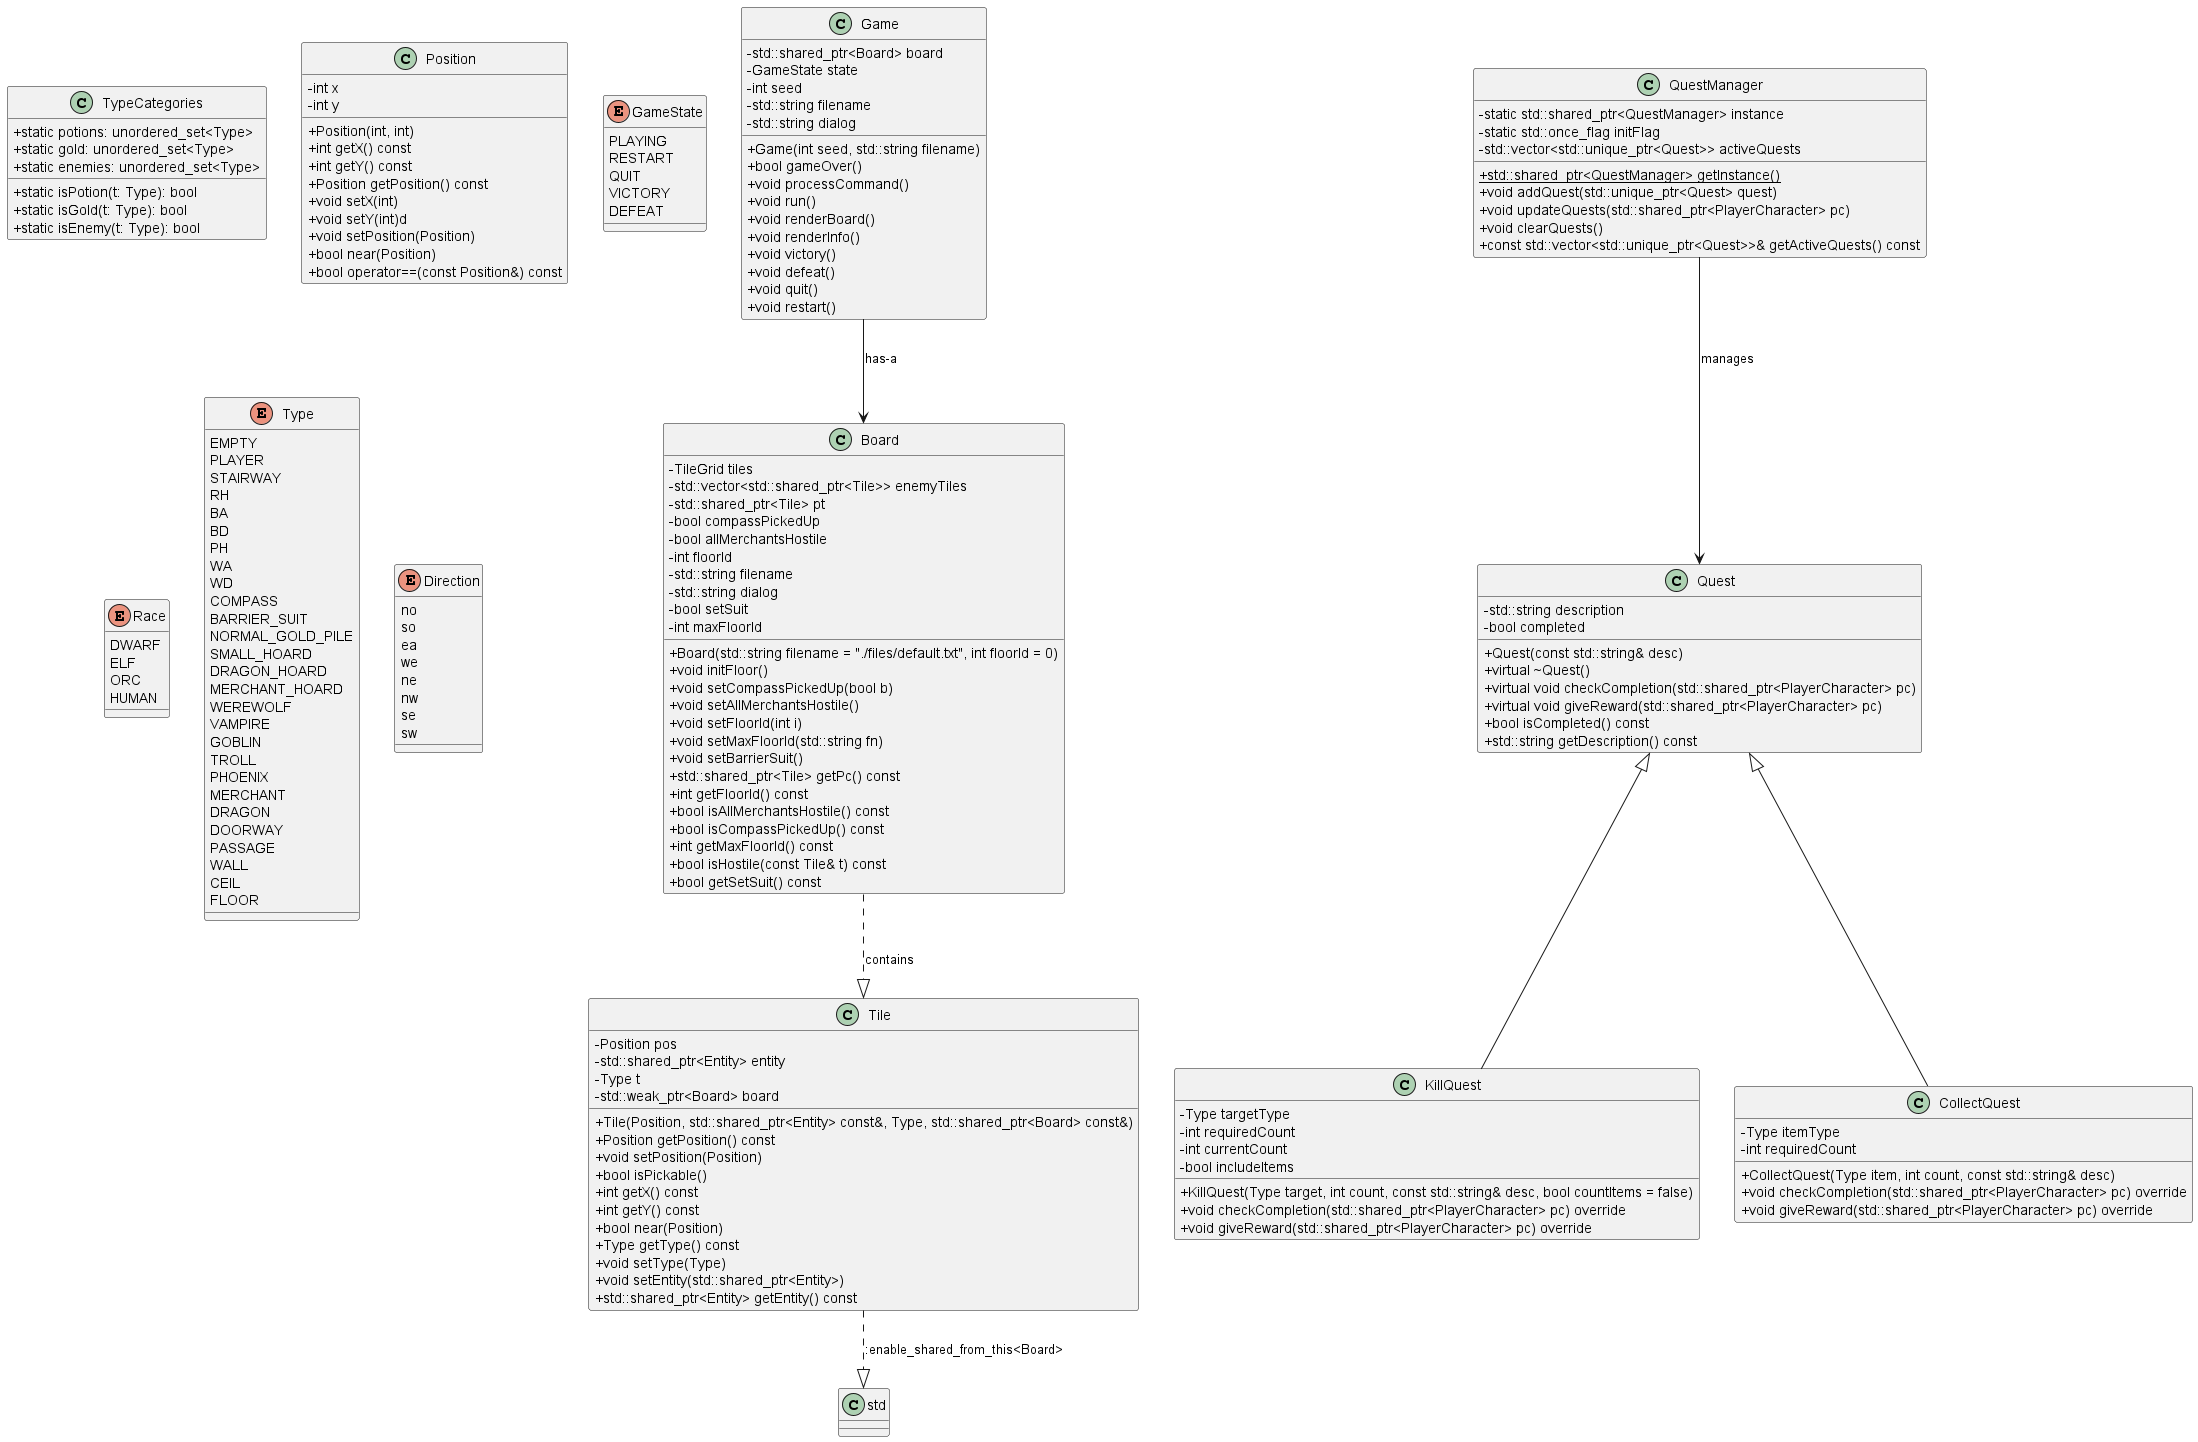
\includegraphics[width=\linewidth]{./out/uml_v1/uml3.png} % Use full line width
    \caption{UML Diagram-3 v1}
    \label{fig:uml-diagram-3}
\end{figure}

\end{document}